\documentclass[12pt,]{article}
\usepackage{lmodern}
\usepackage{setspace}
\setstretch{1}
\usepackage{amssymb,amsmath}
\usepackage{ifxetex,ifluatex}
\usepackage{fixltx2e} % provides \textsubscript
\ifnum 0\ifxetex 1\fi\ifluatex 1\fi=0 % if pdftex
  \usepackage[T1]{fontenc}
  \usepackage[utf8]{inputenc}
\else % if luatex or xelatex
  \ifxetex
    \usepackage{mathspec}
  \else
    \usepackage{fontspec}
  \fi
  \defaultfontfeatures{Ligatures=TeX,Scale=MatchLowercase}
    \setmainfont[]{Noto Serif}
    \setsansfont[]{Noto Sans}
    \usepackage{xeCJK}
    \setCJKmainfont[]{Noto Sans CJK TC}
\fi
% use upquote if available, for straight quotes in verbatim environments
\IfFileExists{upquote.sty}{\usepackage{upquote}}{}
% use microtype if available
\IfFileExists{microtype.sty}{%
\usepackage{microtype}
\UseMicrotypeSet[protrusion]{basicmath} % disable protrusion for tt fonts
}{}
\usepackage[margin=1in]{geometry}
\usepackage{hyperref}
\hypersetup{unicode=true,
            pdftitle={Study Plan for the Financial Assistance Grant for International Students},
            pdfauthor={Thomas Van Hoey 司馬智},
            pdfborder={0 0 0},
            breaklinks=true}
\urlstyle{same}  % don't use monospace font for urls
\usepackage{longtable,booktabs}
\usepackage{graphicx,grffile}
\makeatletter
\def\maxwidth{\ifdim\Gin@nat@width>\linewidth\linewidth\else\Gin@nat@width\fi}
\def\maxheight{\ifdim\Gin@nat@height>\textheight\textheight\else\Gin@nat@height\fi}
\makeatother
% Scale images if necessary, so that they will not overflow the page
% margins by default, and it is still possible to overwrite the defaults
% using explicit options in \includegraphics[width, height, ...]{}
\setkeys{Gin}{width=\maxwidth,height=\maxheight,keepaspectratio}
\IfFileExists{parskip.sty}{%
\usepackage{parskip}
}{% else
\setlength{\parindent}{0pt}
\setlength{\parskip}{6pt plus 2pt minus 1pt}
}
\setlength{\emergencystretch}{3em}  % prevent overfull lines
\providecommand{\tightlist}{%
  \setlength{\itemsep}{0pt}\setlength{\parskip}{0pt}}
\setcounter{secnumdepth}{5}
% Redefines (sub)paragraphs to behave more like sections
\ifx\paragraph\undefined\else
\let\oldparagraph\paragraph
\renewcommand{\paragraph}[1]{\oldparagraph{#1}\mbox{}}
\fi
\ifx\subparagraph\undefined\else
\let\oldsubparagraph\subparagraph
\renewcommand{\subparagraph}[1]{\oldsubparagraph{#1}\mbox{}}
\fi

%%% Use protect on footnotes to avoid problems with footnotes in titles
\let\rmarkdownfootnote\footnote%
\def\footnote{\protect\rmarkdownfootnote}

%%% Change title format to be more compact
\usepackage{titling}

% Create subtitle command for use in maketitle
\newcommand{\subtitle}[1]{
  \posttitle{
    \begin{center}\large#1\end{center}
    }
}

\setlength{\droptitle}{-2em}
  \title{Study Plan for the Financial Assistance Grant for International Students}
  \pretitle{\vspace{\droptitle}\centering\huge}
  \posttitle{\par}
  \author{Thomas Van Hoey 司馬智}
  \preauthor{\centering\large\emph}
  \postauthor{\par}
  \predate{\centering\large\emph}
  \postdate{\par}
  \date{March 2018}




\usepackage{fancyhdr}
\pagestyle{fancy}
\renewcommand{\headrulewidth}{0pt}
\renewcommand{\sectionmark}[1]{\markright{#1}{}}
\fancyhead[LE,RO]{\thepage}
\fancyfoot{}




%- \usepackage{float} #use the 'float' package
%- \floatplacement{figure}{H} #make every figure with caption = h
\usepackage{gb4e}

\usepackage{amsthm}
\newtheorem{theorem}{Theorem}[section]
\newtheorem{lemma}{Lemma}[section]
\theoremstyle{definition}
\newtheorem{definition}{Definition}[section]
\newtheorem{corollary}{Corollary}[section]
\newtheorem{proposition}{Proposition}[section]
\theoremstyle{definition}
\newtheorem{example}{Example}[section]
\theoremstyle{definition}
\newtheorem{exercise}{Exercise}[section]
\theoremstyle{remark}
\newtheorem*{remark}{Remark}
\newtheorem*{solution}{Solution}
\begin{document}
\maketitle
\begin{abstract}
\noindent ``Here is the abstract. Replace the text within the quotation
marks + the quotation marks themselves for the final abstract.''
\par \textbf{Keywords:} a, b
\end{abstract}

\setlength{\parindent}{0.5cm} %#indent
\setlength{\parskip}{0em} %# space between paragraphs

\section{Introduction}\label{introduction}

I have been very grateful to have held the Research Fellowship for
Oustanding International Doctoral Students at National Taiwan University
國立臺灣大學國際優秀博士班學生研究獎助\footnote{This scholarship is now
  renamed the Diaolong Doctoral Scholarship 雕龍國際博士班學生獎助.} for
three years (the maximum period). This financial support helped me
accomplish many academic goals in the past three years (see below and
figure \ref{fig:progress}). However, as shown in the table below, I plan
to finish my doctoral dissertation at the end of the next academic year
(2018-2019). For this reason, I am applying for the Financial Assistance
Grant for International Students provided by National Taiwan University
國立臺灣大學國際學位生助學金.

Below I will show why I believe I am a deserving candidate for the
scholarship. First I will briefly introduce the motivation for my
research. Next I will discuss the desired contributions of my
dissertation. This is followed by the research themes that I have
focused on during my doctoral studies at the Graduate Institute of
Linguistics 語言學研究所 at National Taiwan University thus far,
combined with the key-progress indicators, such as conference
presentations and expected publications. Lastly, I provide a tentative
timetable, which I intend to follow during next academic year. I believe
that with the support of the Financial Assistance Grant for
International Students, I can complete my PhD dissertation in a timely
fashion.

\section{The motivation for my
research}\label{the-motivation-for-my-research}

The last three decades have seen a renewed interest in reexamining the
Saussurean dictum that the link between meaning and form in language is
arbitrary. That is to say, there has been much research on iconicity
(esp. in Cognitive Linguistics). Two of the most salient subfields that
have to do with iconicity are sound symbolism (Hinton, Nichols \& Ohala
1994) and ideophones (Voeltz \& Kilian-Hatz 2001).

Ideophones, defined as `marked words that depict sensory image'
(Dingemanse 2011; 2012), occur very frequently in Chinese; see, for
example, Mok (2001); Lu 呂 (2006); Meng (2012); Wu (2014); and Van Hoey
(2015). In Chinese, these words are more commonly known as onomatopoeia
(\emph{nishengci} 擬聲詞 or \emph{xiangshengci} 象聲詞) when they depict
sound. However, Chinese ideophones are semantically very rich and can
also depict other sensory modalities like vision, motion, texture,
temperature, inner feelings, evaluation etc. (termed `\emph{nitaici}'
擬態詞) --- a dimension of their semantics that is not as well-known as
that of other East-Asian languages, e.g.~Japanese and Korean.

My research is focused on their development throughout time and studies
Chinese ideophones from a maximalist perspective, while keeping
up-to-date with relevant research in other domains, by engaging with
other scholars at conferences and the studies they performed. For
instance, in 2017 I was able to go to the Netherlands as well as to
Japan to meet experts in my field of linguistic iconicity.

\section{Contributions of my
dissertation}\label{contributions-of-my-dissertation}

First, my \textbf{interdisciplinary research} is innovative because it
incorporates theories and evidence from different academic fields in
order to study ideophones in Chinese, e.g.~linguistics, cultural
studies, and cognitive science. While most recent research on ideophones
limits its scope to synchronic study (i.e.~ideophones as they occur in
current language use), but because of digitization projects of Chinese,
e.g.~the Academia Sinica corpora, I am able to investigate \textbf{the
development of Chinese ideophones through time} and offer an almost
unique perspective to my field.

Second, I am working on a \textbf{consultable database} to handle the
different kinds of data which ultimately should become a tool for
further research of this overlooked set of words in Chinese. As of now,
I have identified 784 different types of ideophones, and I believe many
more are to be found. Furthermore, the database can be used as a
starting point for future corpus-based research. I am constructing it as
part of the \textbf{digital humanities} movement and in the hope of
promoting \textbf{reproducible research}.

Third, recent research (Perniss \& Vigliocco 2014; Lockwood \&
Dingemanse 2015) focuses on \textbf{linguistic synaesthesia}, i.e.~when
ideophones express more than one sensory modality at the same time. This
still is, however, an often neglected point in ideophone research that
is only recently becoming a hot topic, and I want to share my Chinese
data with the research community in order to improve our understanding
of ideophones in general.

\section{Four research themes and key-progress
indicators}\label{four-research-themes-and-key-progress-indicators}

My MA thesis (Van Hoey 2015) at the Catholic University of Leuven
(魯汶大學), Belgium, investigated ideophones in Tang-dynasty Middle
Chinese. Since starting my doctoral studies at NTU (Fall 2015), I have
mainly focused on the \textbf{historical development of ideophones} in
Pre-Modern Chinese. The first in-depth study I conducted at NTU was an
investigation of ideophones in the \emph{Shijing} 詩經, presented at
ISACG 9 in Berlin (Van Hoey 2016a). This study was complementary to my
MA thesis, since they were both collections of poetry and songs.\\
However, last year I developed an interest in other genres as well, and
developed a methodology for studying the functional usage of ideophones
in historical texts, with a case study on the \emph{Three Histories}
三史. I presented this paper as an invited speaker at the Mimetics 2
Workshop in Nagoya (Van Hoey 2017b).

A second theme in my research has been \textbf{variation} of ideophones.
At the CLDC 8 conference, organised at NTU, I presented (with my advisor
Dr.~Lu Chiarung) a study on three variant ideophones---\emph{mángmáng}
芒芒, \emph{mángmáng} 茫茫, and \emph{cāngmáng} 蒼茫---that roughly had
the same meaning of `broad, wide' and provided reasons for why
\emph{mángmáng} 茫茫 came out as the one still in use today (Van Hoey \&
Lu 2016). This paper will be published in the CLR series (Van Hoey \& Lu
to appear). For this year's ICPEAL 17 - CLDC 9 joint conference, we are
submitting a paper on the development of ideophones that depict
\textsc{light}, e.g. \emph{yìyì} 熠熠, \emph{cànlàn} 燦爛, or
\emph{shǎnshǎn} 閃閃 (Van Hoey \& Lu awaiting submission result).

The third focus of my doctoral research has been \textbf{typology}. In
2015 I undertook a study on meteorological expressions in Mandarin
Chinese, which also focused on weather-related ideophones, and presented
at the Max Planck Institute for Psycholinguistics (Netherlands) (Van
Hoey 2017a). This paper I recently submitted to the \emph{Journal of
Cognitive Semantics} and I am awaiting their review (Van Hoey under
review). The second typology-related study is a paper that compares the
semantic domains of ideophones across languages. The semantic map, which
I first presented in Tachikawa, Japan (Van Hoey 2016b), is in
preparation for journal submission. The manuscript, however, has already
been found useful by another PhD student at the University of Hong Kong
who is also exploring iconicity, and they have cited it in a paper they
are preparing for publication as well.

Finally, the most recent theme in my research is the \textbf{acquisition
of ideophones}. This theme is still in its infancy, but I want to
investigate how (young) native speakers of Chinese learn onomatopoeia
and reduplication, and to what degree. I currently view this theme as
supplementary to the historical data that dominate most of my research.
That is to say, since I have no native speakers of Classical Chinese who
I can consult for experiments or intuition, I hope to be able to
converge acquisition-based evidence with historical evidence to get a
well-rounded understanding of ideophones in Chinese.

\begin{figure}
\centering
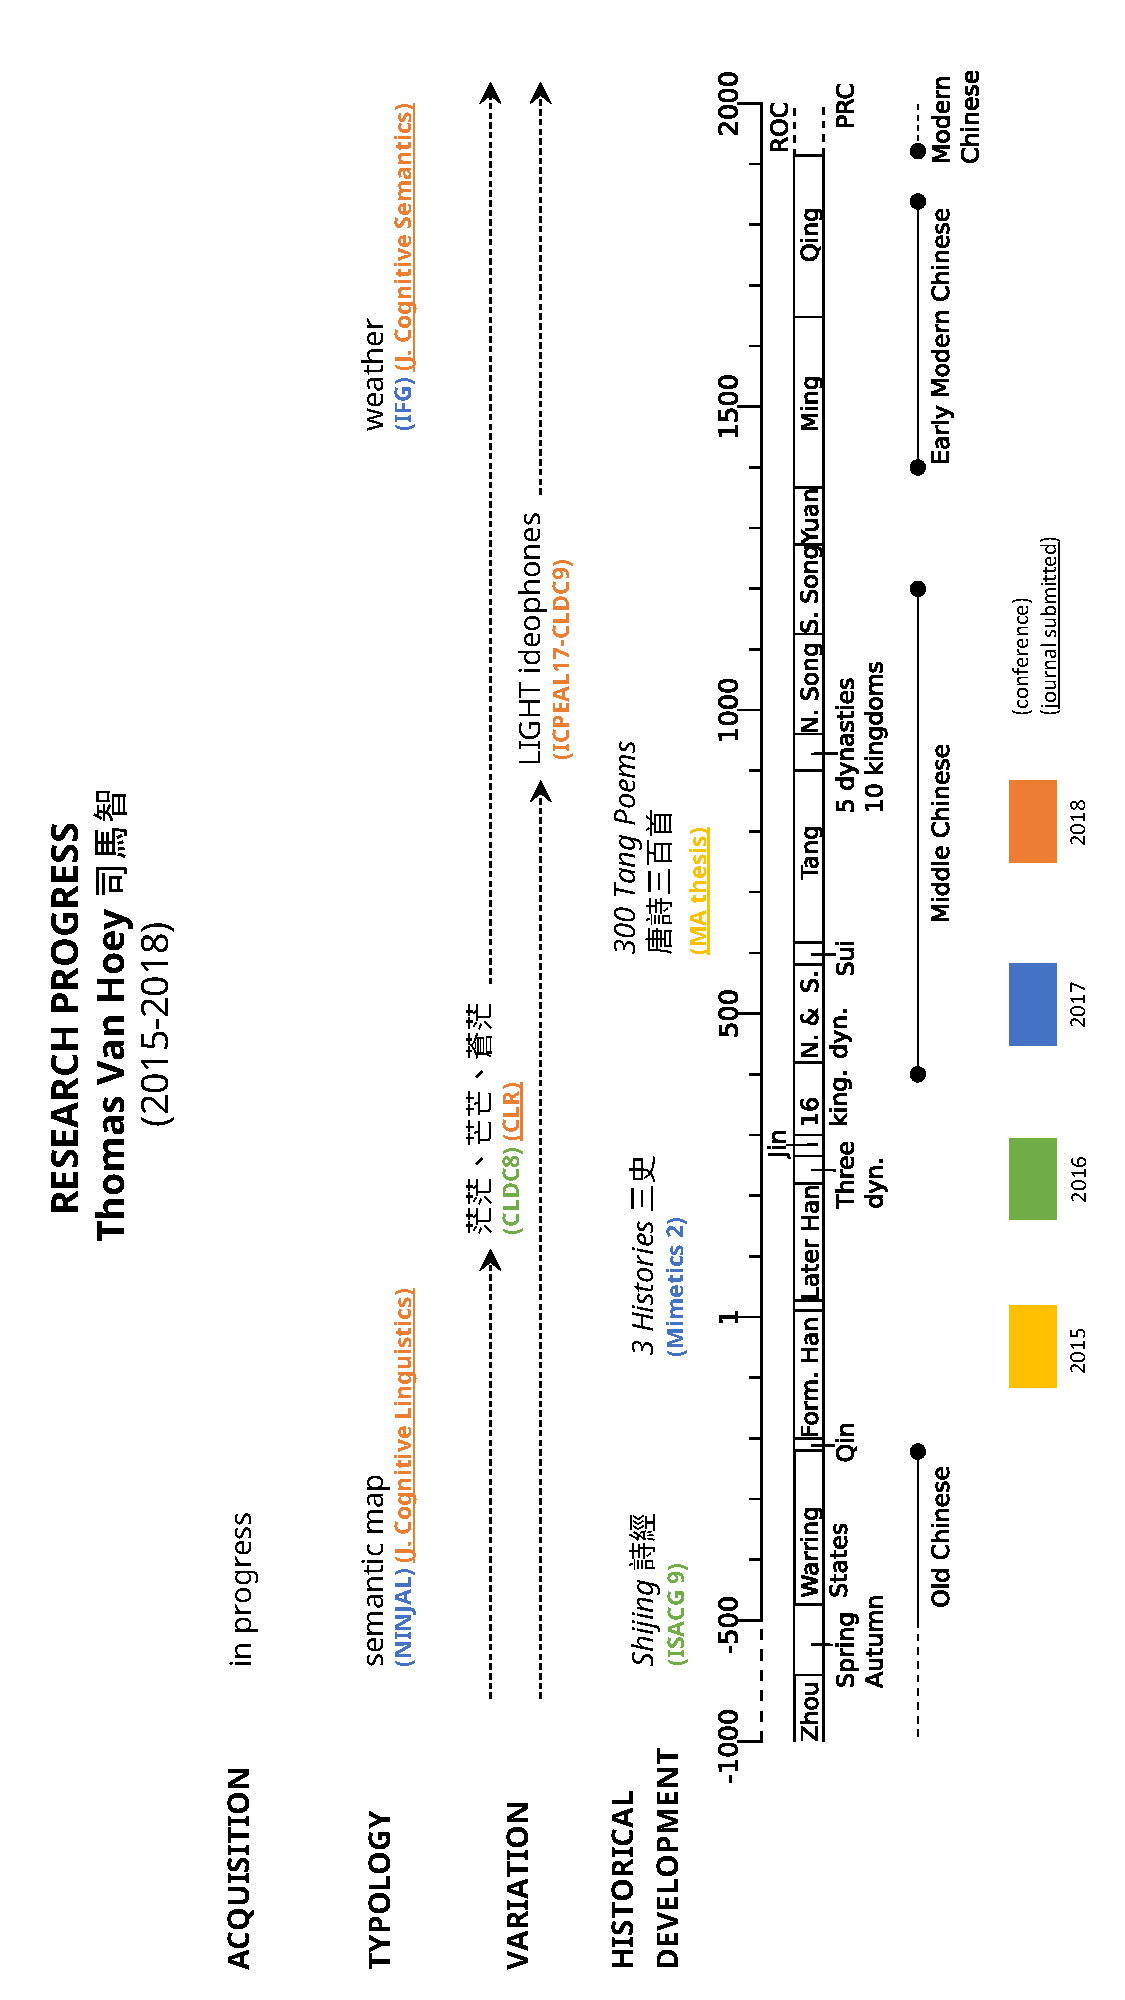
\includegraphics{progress.pdf}
\caption{\label{fig:progress}Research progress Thomas Van Hoey (2015-2018)}
\end{figure}

\section{Tentative timetable}\label{tentative-timetable}

\begin{longtable}[]{@{}cccc@{}}
\toprule
\begin{minipage}[b]{0.20\columnwidth}\centering\strut
time\strut
\end{minipage} & \begin{minipage}[b]{0.26\columnwidth}\centering\strut
goal\strut
\end{minipage} & \begin{minipage}[b]{0.18\columnwidth}\centering\strut
時間\strut
\end{minipage} & \begin{minipage}[b]{0.24\columnwidth}\centering\strut
目標\strut
\end{minipage}\tabularnewline
\midrule
\endhead
\begin{minipage}[t]{0.20\columnwidth}\centering\strut
July-August 2018\strut
\end{minipage} & \begin{minipage}[t]{0.26\columnwidth}\centering\strut
write proposal\strut
\end{minipage} & \begin{minipage}[t]{0.18\columnwidth}\centering\strut
2018年7-8月\strut
\end{minipage} & \begin{minipage}[t]{0.24\columnwidth}\centering\strut
寫論文計畫書\strut
\end{minipage}\tabularnewline
\begin{minipage}[t]{0.20\columnwidth}\centering\strut
September 2018\strut
\end{minipage} & \begin{minipage}[t]{0.26\columnwidth}\centering\strut
get QPPQ publication requirement\strut
\end{minipage} & \begin{minipage}[t]{0.18\columnwidth}\centering\strut
2018年9月\strut
\end{minipage} & \begin{minipage}[t]{0.24\columnwidth}\centering\strut
符合資格論文要求\strut
\end{minipage}\tabularnewline
\begin{minipage}[t]{0.20\columnwidth}\centering\strut
October 2018\strut
\end{minipage} & \begin{minipage}[t]{0.26\columnwidth}\centering\strut
defend proposal\strut
\end{minipage} & \begin{minipage}[t]{0.18\columnwidth}\centering\strut
2018年10月\strut
\end{minipage} & \begin{minipage}[t]{0.24\columnwidth}\centering\strut
論文計畫書口試\strut
\end{minipage}\tabularnewline
\begin{minipage}[t]{0.20\columnwidth}\centering\strut
October 2018\strut
\end{minipage} & \begin{minipage}[t]{0.26\columnwidth}\centering\strut
ICPEAL 17-CLDC 9 conference\strut
\end{minipage} & \begin{minipage}[t]{0.18\columnwidth}\centering\strut
2018年10月\strut
\end{minipage} & \begin{minipage}[t]{0.24\columnwidth}\centering\strut
參與ICPEAL 17-CLDC 9 國際研討會\strut
\end{minipage}\tabularnewline
\begin{minipage}[t]{0.20\columnwidth}\centering\strut
November 2018- March 2019\strut
\end{minipage} & \begin{minipage}[t]{0.26\columnwidth}\centering\strut
finish 1st draft of dissertation\strut
\end{minipage} & \begin{minipage}[t]{0.18\columnwidth}\centering\strut
2018年11月 至2019年3月\strut
\end{minipage} & \begin{minipage}[t]{0.24\columnwidth}\centering\strut
寫好博士論文草稿\strut
\end{minipage}\tabularnewline
\begin{minipage}[t]{0.20\columnwidth}\centering\strut
March-May 2019\strut
\end{minipage} & \begin{minipage}[t]{0.26\columnwidth}\centering\strut
final draft dissertation\strut
\end{minipage} & \begin{minipage}[t]{0.18\columnwidth}\centering\strut
2019年3-5月\strut
\end{minipage} & \begin{minipage}[t]{0.24\columnwidth}\centering\strut
寫好博士論文\strut
\end{minipage}\tabularnewline
\begin{minipage}[t]{0.20\columnwidth}\centering\strut
June/July 2019\strut
\end{minipage} & \begin{minipage}[t]{0.26\columnwidth}\centering\strut
oral defense\strut
\end{minipage} & \begin{minipage}[t]{0.18\columnwidth}\centering\strut
2019年6-7月\strut
\end{minipage} & \begin{minipage}[t]{0.24\columnwidth}\centering\strut
博士論文口試\strut
\end{minipage}\tabularnewline
\begin{minipage}[t]{0.20\columnwidth}\centering\strut
July-August 2019\strut
\end{minipage} & \begin{minipage}[t]{0.26\columnwidth}\centering\strut
revisions of dissertation\strut
\end{minipage} & \begin{minipage}[t]{0.18\columnwidth}\centering\strut
2019年7-8月\strut
\end{minipage} & \begin{minipage}[t]{0.24\columnwidth}\centering\strut
博士論文修改\strut
\end{minipage}\tabularnewline
\bottomrule
\end{longtable}

\section{References}\label{references}

\setlength{\parindent}{-0.5in} \setlength{\leftskip}{0.5in}
\setlength{\parskip}{8pt} \noindent

\hypertarget{refs}{}
\hypertarget{ref-Dingemanse2011a}{}
Dingemanse, Mark. 2011. The meaning and use of ideophones in Siwu.
Nijmegen: Radboud University Nijmegen Dissertation.

\hypertarget{ref-Dingemanse2012}{}
Dingemanse, Mark. 2012. Advances in the cross-linguistic study of
ideophones. \emph{Language and Linguistics Compass} 6(10). 654--672.

\hypertarget{ref-Hinton1994}{}
Hinton, Leanne, Johanna Nichols \& John J. Ohala (eds.). 1994.
\emph{Sound symbolism}. Cambridge {[}England{]} ; New York, NY:
Cambridge University Press.

\hypertarget{ref-Lockwood2015a}{}
Lockwood, Gwilym \& Mark Dingemanse. 2015. Iconicity in the lab: A
review of behavioral, developmental, and neuroimaging research into
sound-symbolism. \emph{Frontiers in Psychology} 6(1246). 1--14.
doi:\href{https://doi.org/10.3389/fpsyg.2015.01246}{10.3389/fpsyg.2015.01246}.
\url{http://journal.frontiersin.org/Article/10.3389/fpsyg.2015.01246/abstract}
(4 December, 2017).

\hypertarget{ref-Meng2012}{}
Meng, Chenxi. 2012. A description of ideophonic words in Mandarin
Chinese. Leiden: Leiden University Research Master in Linguistics.

\hypertarget{ref-Mok2001}{}
Mok, Waiching Enid. 2001. Chinese sound symbolism: A phonological
perspective. Hawai'i: University of Hawai'i PhD Dissertation.

\hypertarget{ref-Perniss2014}{}
Perniss, Pamela \& Gabriella Vigliocco. 2014. The bridge of iconicity:
Form a world of experience to the experience of language.
\emph{Philosophical transactions of The Royal Society} 369. 1--13.

\hypertarget{ref-VanHoey2015}{}
Van Hoey, Thomas. 2015. Ideophones in Middle Chinese: A typological
study of a Tang dynasty poetic corpus. Leuven: KU Leuven Master Thesis.

\hypertarget{ref-VanHoey2016a}{}
Van Hoey, Thomas. 2016a. Ideophones in Old Chinese: The case of the
Shijing 詩經. In, \emph{ISACG 9 {[}International Symposium on Ancient
Chinese Grammar{]}}. Berlin: Humboldt University.

\hypertarget{ref-VanHoey2016b}{}
Van Hoey, Thomas. 2016b. Ideophones in Premodern Chinese: Revisiting
Dingemanse's implicational hierarchy (poster). In, \emph{Mimetics in
Japanese and other languages in the world
(日本語と世界諸言語のオノマトペ)}. Tachikawa: NINJAL.

\hypertarget{ref-VanHoey2017}{}
Van Hoey, Thomas. 2017a. The thunder rolls: Iconicity and ideophones in
Chinese meteorological expressions. In, \emph{CLS-MPI Iconicity Focus
Group Workshop: Types of Iconicity in Language Use, Development and
Processing}. Nijmegen: Max Planck Institute for Psycholinguistics.

\hypertarget{ref-VanHoey2017a}{}
Van Hoey, Thomas. 2017b. Chinese ideophones in historical corpora: A
case study of mental space markers. In, \emph{Workshop on Mimetics II:
New approaches to old questions}. Nagoya: Nanzan University.

\hypertarget{ref-VanHoeyunderreviewa}{}
Van Hoey, Thomas. under review. Does the thunder roll? Mandarin Chinese
meteorological expressions and their iconicity. \emph{Journal of
Cognitive Semantics}.

\hypertarget{ref-VanHoey2016c}{}
Van Hoey, Thomas \& Chiarung Lu. 2016. The distribution of ideophones in
Tang poems: A variationist perspective. In, \emph{CLDC 8 {[}Conference
on Language, Discourse, and Cognition{]}}. Taipei: National Taiwan
University.

\hypertarget{ref-VanHoeyawaitingsubmissionresult}{}
Van Hoey, Thomas \& Chiarung Lu. awaiting submission result. All that
glitters is not gold: Prototypical semantic change in shiny Literary
Chinese ideophones. In, \emph{Workshop on Mimetics II: New approaches to
old questions}. Nagoya: National Taiwan University.

\hypertarget{ref-VanHoeytoappear}{}
Van Hoey, Thomas \& Chiarung Lu. to appear. Ideophones in Chinese
classics: Their development and distribution from a variationist
perspective. ms.

\hypertarget{ref-Voeltz2001}{}
Voeltz, Erhard Friedrich Karl \& Christa Kilian-Hatz (eds.). 2001.
\emph{Ideophones}. (Typological Studies in Language v. 44). Amsterdam ;
Philadelphia: J. Benjamins.

\hypertarget{ref-Wu2014}{}
Wu, Mengqi. 2014. The structure of ideophones in Southern Sinitic. Hong
Kong: University of Hong Kong Master Thesis.

\hypertarget{ref-Lu2006}{}
呂, 佳蓉. 2006.
擬音語・擬態語の比喩的拡張の諸相――認知言語学と類型論の観点から. Giongo,
gitaigo no hiyuteki kakuchō no shosō: ninchi gengogaku to reikeiron no
kanten kara. Kyōto: Kyōto University PhD dissertation.


\end{document}
